\documentclass[12pt]{article}

\usepackage[utf8]{inputenc}
\usepackage[T1]{fontenc}
\usepackage[francais]{babel}

\title{\textbf{TP \#19 - Etude du fonctionnement d'une pile, réaction d'oxydoréduction}}
\date{}
\usepackage{graphicx}
\begin{document}

\maketitle

\section{}
\section{Etude d'une pile Fer-Cuivre}

\begin{figure}[htp]
\centering
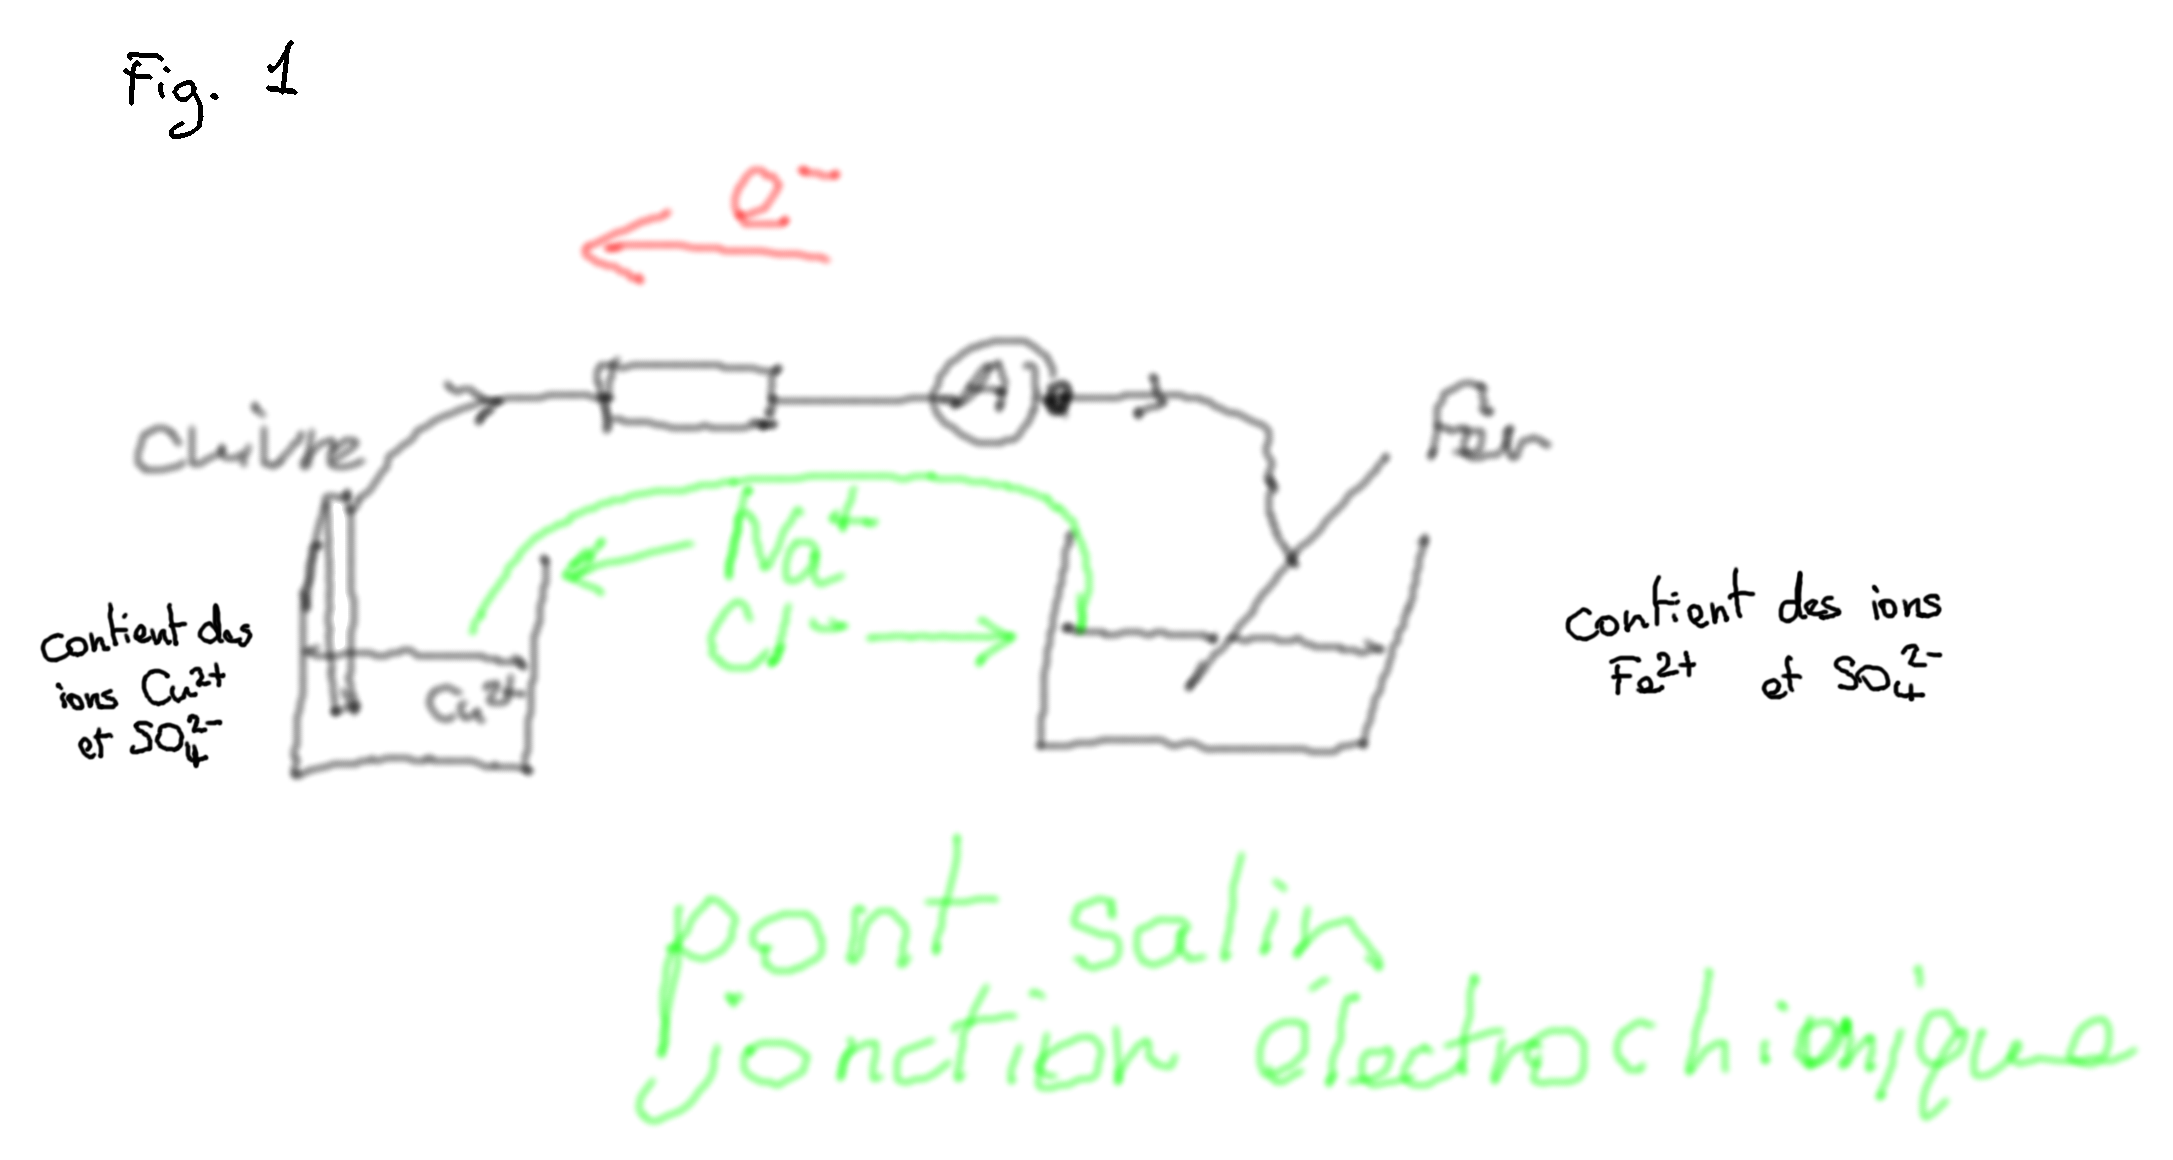
\includegraphics[scale=0.9]{img/tp19_fig1.png}
\caption{Etude d'une pile Fer-Cuivre}
\label{}
\end{figure}

Pont salin : papier imbibé d'eau salé (= jonction électrochimique)

Réactifs : $Fe + Cu^{2+}$ \\
Produits : $Cu$

Equation de réaction : $Cu^{2+} + Fe \rightarrow Cu + Fe^{2+}$

Il y a eu échange d'électrons lors de cette réaction entre $Fe$ et $Cu^{2+}$ par contact direct.

Or dans la pile la même réaction a lieu mais les réactifs n sont pas en contact.

Les électrons circulent via les fils électriques (d'où le courant).

Demi-équations :
\begin{itemize}
\item A l'électrode de $Fe$ : $Fe = Fe^{2+} + 2e^-$
\item A l'électrode de $Cu$ : $Cu^{2+} + 2e^- = Cu$
\end{itemize}

Equation globale : $Fe_{(s)} + Cu^{2+}_{(aq)} \rightarrow Cu_{(s)} + Fe^{2+}_{(aq)}$

\begin{itemize}
\item Au pôle - : une réaction produit des électrons
\item Au pôle + : une réaction consomme des électrons
\end{itemize}

\textbf{Circulation des ions dans le pont salin}

Dans le compartiment de cuivre :
\begin{itemize}
\item La lame de cuivre reçoit des électrons
\item Les électrons sont consommés par les ions $Cu^{2+}$ et se transforment en atomes $Cu$
\item Disparition d'ions $Cu^{2+}$. La solution n'est donc plus neutre (elle est négative).
=> Pour que la solution reste neutre, il faut que des cathions $Na^+$ se déplacent vers la solution. D'où le sens de circulation des ions $Na^+$.
\end{itemize}

Pour le fer :
\begin{itemize}
\item La lame donne des électrons
\item Des électrons de Fe se transforment en ions $Fe^{2+}$
\item Augmentation du nombre de cathions
=> Pour que la solution reste neutre, il faut que des anions $Cl^-$ se déplacent vers la solution.
\end{itemize}

\section{Les réactions d'oxydoréduction}

\emph{Apprendre par coeur les définitions !}

\begin{figure}[htp]
\centering
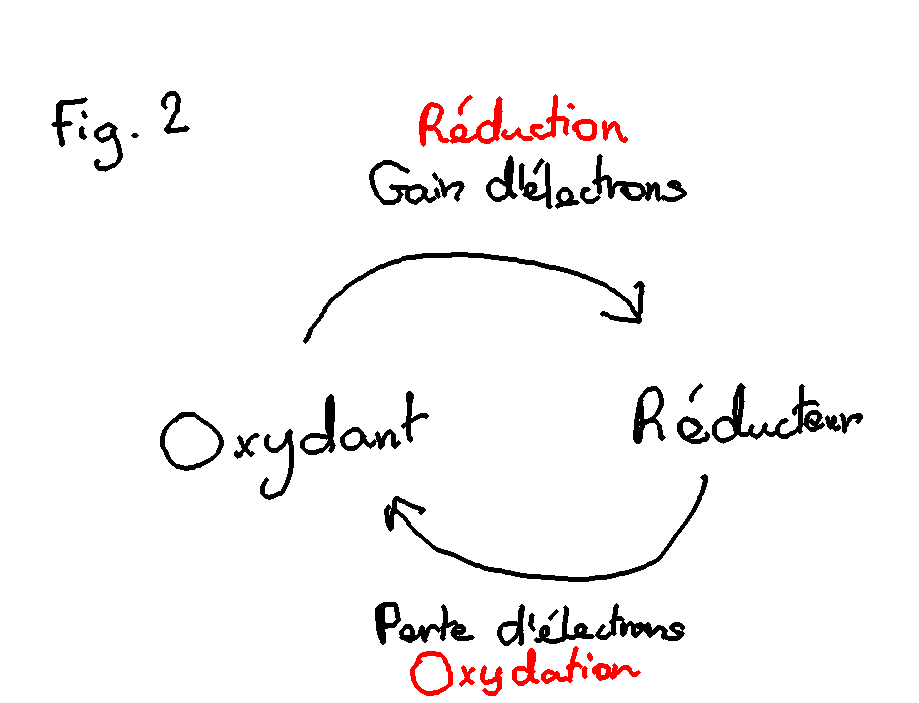
\includegraphics[scale=1.00]{img/tp19_fig2.png}
\caption{Les réactions d'oxydoréduction}
\label{}
\end{figure}

\[Ox + ne^- = Red\]

L'ion $Cu^{2+}$ (oxydant) GAGNE $2e^-$ et se transforme en $Cu$ (réducteur).
\textbf{L'oxydant de la pile est l'ion $Cu^{2+}$.}

Le fer (réducteur) PERD $2e^-$ et se trandforme en $Fe^{2+}$ (oxydant).
\textbf{Le réducteur de la pile est l'atome de $Fe$.}

NB : l'oxydant et le réducteur de la réaction font partie des réactifs.

L'ion $Cu^{2+}$ subit une réduction.\\
L'atome de $Fe$ subit une oxydation.

En chimie : \emph{conjugué} synonyme d'\emph{associé}. Ex de couples :
\begin{itemize}
\item $Fe^{2+}$ / $Fe$
\item $Fe^{3+}$ / $Fe^{2+}$
\item $Cu^{2+}$ / $Cu$
\item \textbf{Oxydant / réducteur}
\end{itemize}

\textbf{Etablir une équation d'oxydoréduction}

$MnO_4^-$ et $Fe^{2+}$

Couples :
\begin{itemize}
\item \textbf{$MnO_4^-$} / $Mn^{2+}$
\item $Fe^{3+}$ / \textbf{$Fe^{2+}$}
\end{itemize}

Demi-équations :
\begin{itemize}
\item $8H^+ + MnO_{4_{(aq)}}^- + 5e^- = Mn^{2+}_{(aq)} + 4H_2O$ (les ions sont en solution aqueuse $\rightarrow$ on peut équilibrer l'équation avec de l'eau et des ions H+, présents naturellement)
\end{itemize}

\end{document}